\section{Esperimenti sull’architettura e sulla funzione di loss}

Non soddisfatti dei risultati abbiamo cambiato l'architettura della rete,
passando a 7 layer di convoluzione, lavorando sempre sul canale Y.

\subsection{Modifiche per fase di training}

Il numero di patch estratte per immagine durante il training è stato aumentato da 20 a 40,
ottenute dal dataset DIV2K di 800 immagini, portando il numero totale di campioni a circa 32 mila.
La grandezza delle patch è stata aumentata da 64 a 128,
in modo di permettere alla rete di vedere più informazioni.

\subsection{Modifiche all'architettura}
Il primo layer di convoluzione ha un kernel di $9\times9$ mentre i
restanti hanno kernel con grandezza $3\times3$.
Come loss function abbiamo mantenuto la MSE tra l'immagine di output
dalla rete e la ground truth, ovvero l'immagine ad alta risoluzione.
Il learning rate è stato fissato a $10^{-4}$ per tutti i layer stavolta.

Aumentando il numero di layer ci aspettiamo di
ottenere potenziali miglioramenti per quanto riguarda l'output della rete.

Abbiamo inserito anche un early stopping per evitare di sprecare tempo durante la fase di training, se la rete non migliora il proprio PSNR globale per 120 epoche consecutive il training si ferma.

Con questa nuova architettura ci siamo avvicinati ai valori PSNR dell'algoritmo bicubic ma ancora non abbastanza da poter superarlo.

È stato inoltre valutato il residual learning.
In questo approccio, la rete non apprende direttamente la mappatura dall’immagine a bassa risoluzione (LR) a quella ad alta risoluzione (HR),
ma la differenza residua tra le due.
In questo modo il modello non modifica la struttura dell’architettura in senso ResNet,
ma cambia semplicemente la quantità che la rete è chiamata a stimare.

Questi cambiamenti sono stati presi dal paper VDSR \cite{kim2015accurate}.

\begin{figure}[ht]
    \centering

    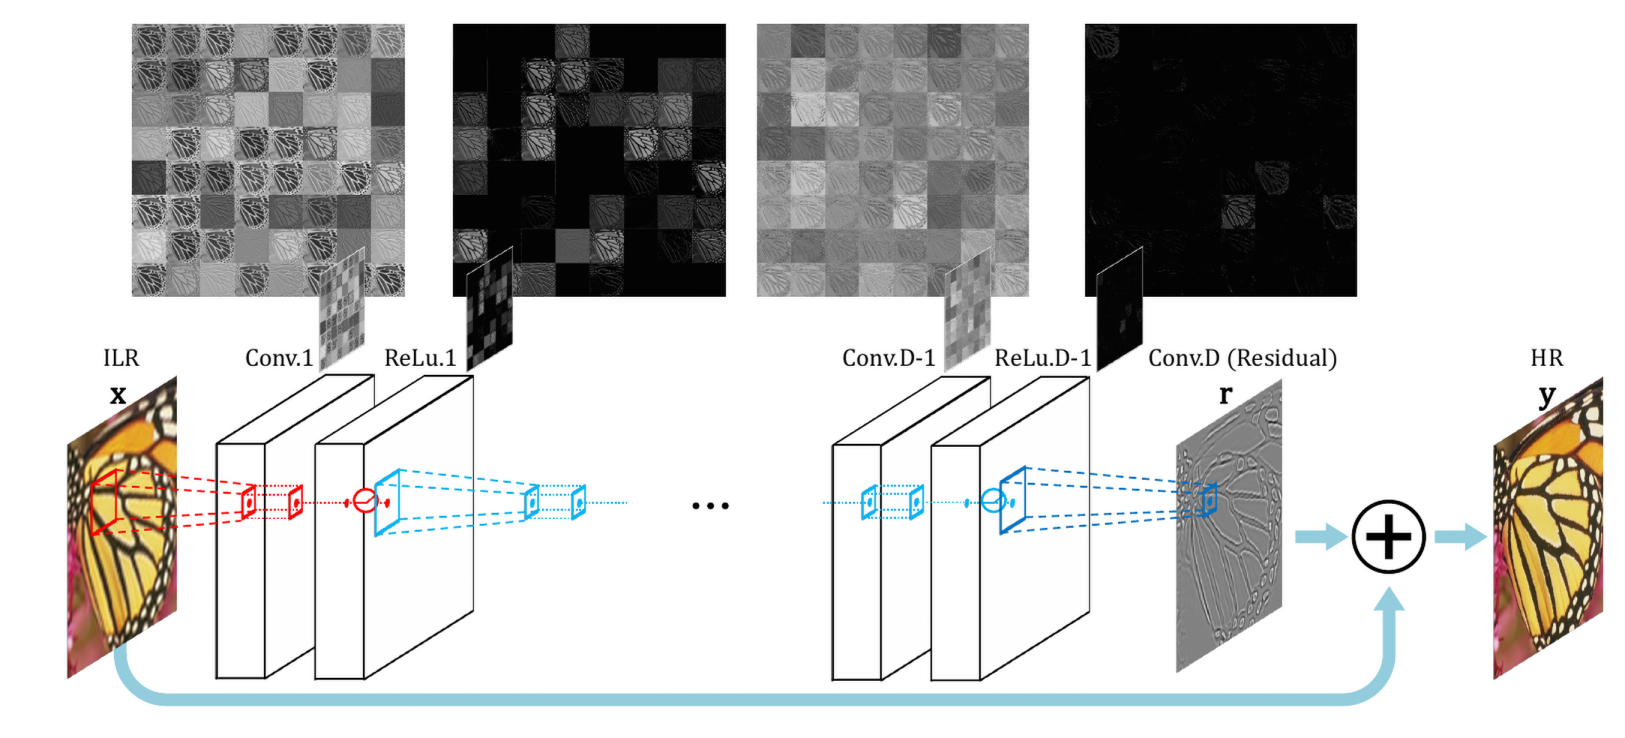
\includegraphics[width=1\columnwidth]{figures/architettura_VDSR.png}
    \caption{Architettura rete VDSR}

\end{figure}

\subsection{Differenze con paper VDSR \cite{kim2015accurate}}

Una differenza sostanziale rispetto al modello VDSR \cite{kim2015accurate} riguarda la profondità della rete:
quest’ultimo utilizza 20 layer convoluzionali, mentre nel nostro caso ne sono stati impiegati 7,
al fine di ottenere risultati soddisfacenti in tempi di addestramento più contenuti.

Con questa architettura sono stati ottenuti risultati migliori rispetto al modello SRCNN \cite{dong2014srcnn}.
Tuttavia, in nessuna istanza del test set si è riusciti a superare le prestazioni dell’interpolazione bicubica.

Con questa architettura è stata osservata una variazione instabile del PSNR durante la fase di training.
Per ridurre tale instabilità è stata introdotta la batch normalization dopo ogni layer convoluzionale,
al fine di normalizzare le attivazioni intermedie della rete e stabilizzare il processo di ottimizzazione.

L’introduzione della batch normalization ha portato a una riduzione
delle oscillazioni
del PSNR durante il training; anche questa scelta si discosta da VDSR\cite{kim2015accurate}.

Abbiamo inoltre cambiato la grandezza dei kernel dal
layer 2 al layer 7 da $3\times3$ a $5\times5$, in modo da osservare eventuali
miglioramenti nei risultati, anche se questo si discosta dal paper VDSR \cite{kim2015accurate}
che usava $3\times3$ come grandezza per i kernel dei layer intermedi.


Come ultimo tentativo abbiamo provato a sostituire MSE come funzione di loss con L1.
La MSE eleva al quadrato la differenza penalizzando di
più errori grandi rispetto a quelli piccoli, L1 invece prende il valore assoluto,
dando lo stesso peso a tutti gli errori commessi dalla rete.

\subsection{Risultati finali}

\begin{figure}[ht]
    \centering

    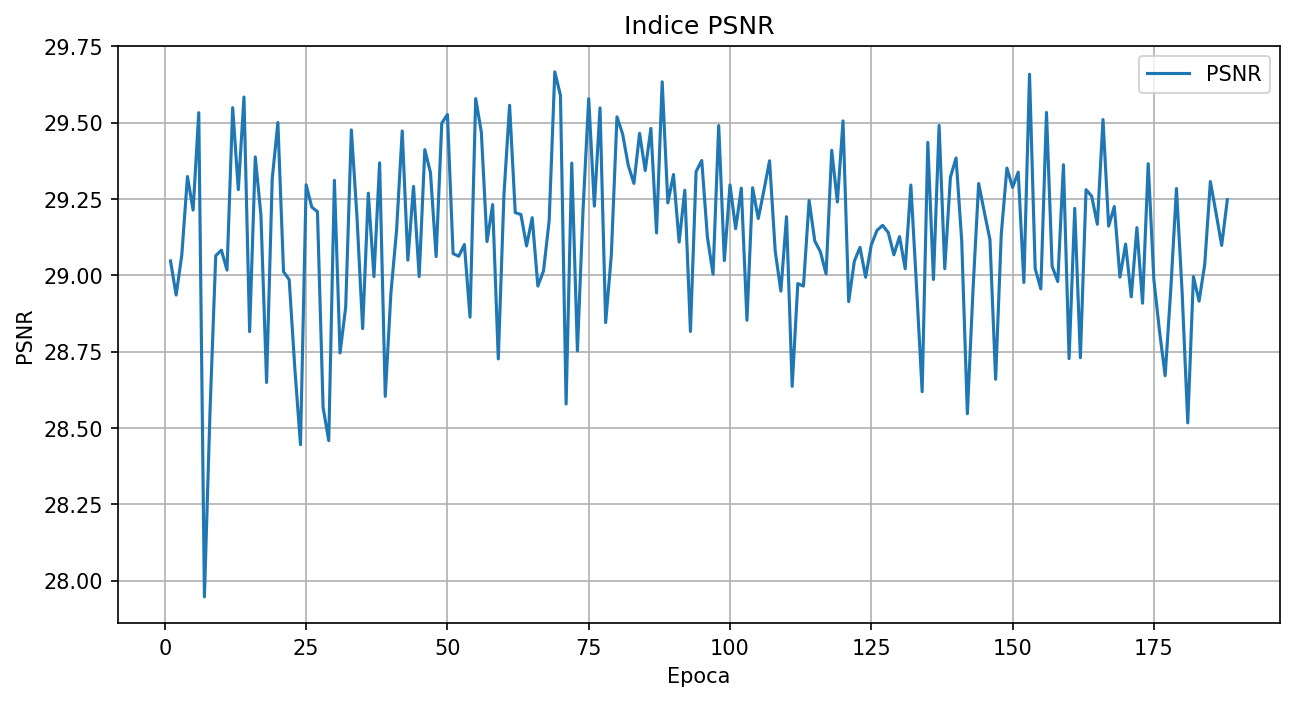
\includegraphics[width=0.8\columnwidth]{figures/srcnn_600_9-3-3-3-3-3-3_psnr_plot.png}
    \caption{Kernel: 3x3; no BN, MSE Loss}

    \vspace{0.5cm}

    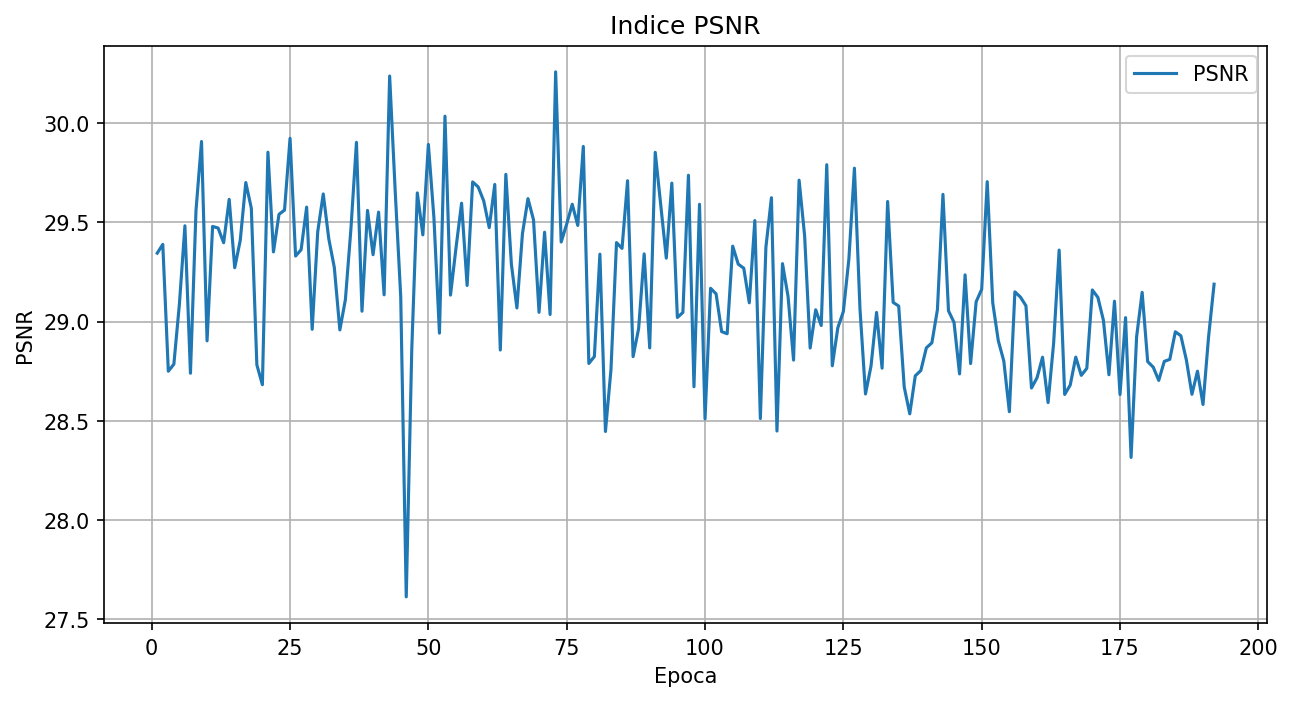
\includegraphics[width=0.8\columnwidth]{figures/srcnn_600_9-5-5-5-5-5-5_BN_L1_psnr_plot.png}
    \caption{Kernel: 5x5, BN, L1 Loss}

\end{figure}

Grazie alla loss L1 siamo riusciti a superare l'algoritmo Bicubic in una istanza del test set,
ottenendo anche un miglioramento  sui dettagli dell'immagine visibile ad occhio nudo.

\begin{figure}[ht]
    \centering
    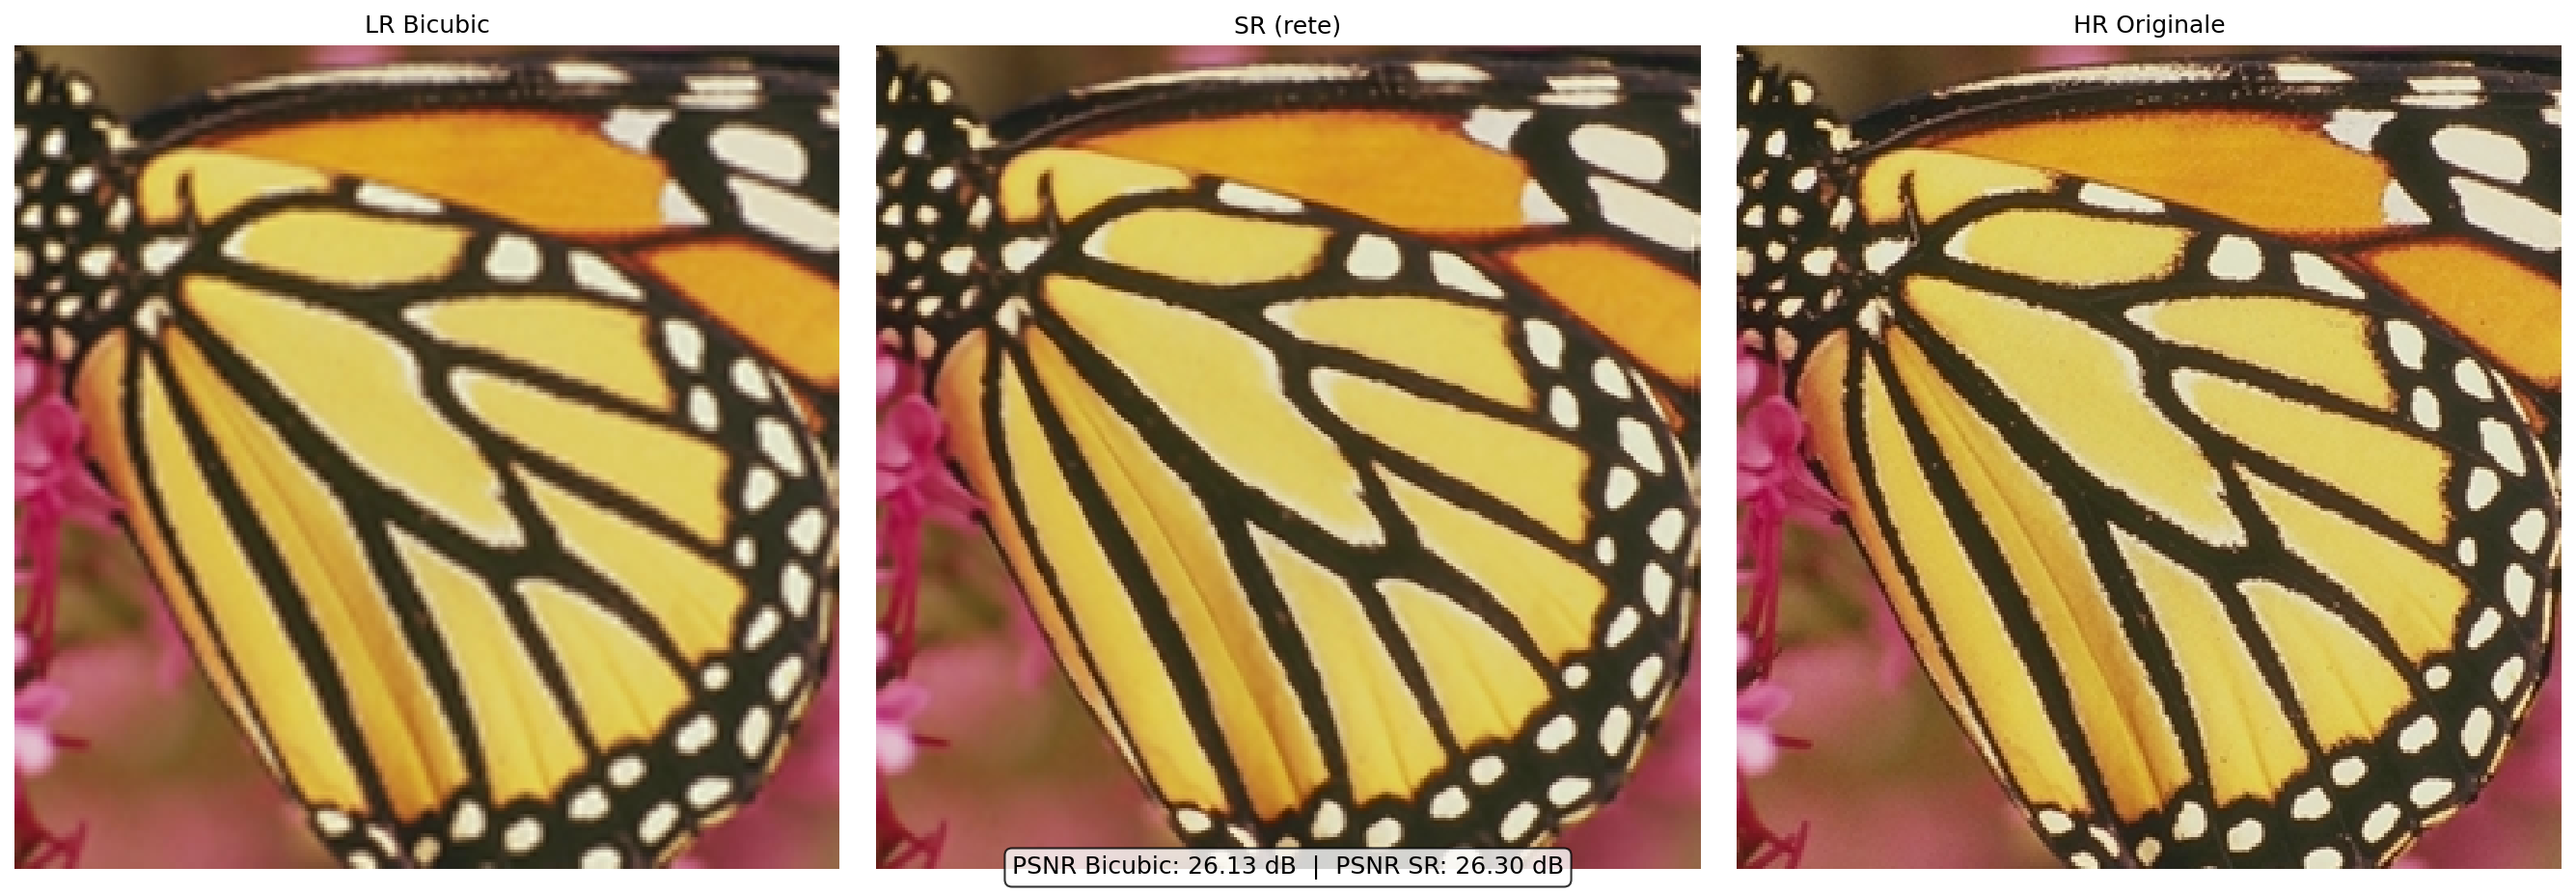
\includegraphics[width=\columnwidth]{figures/risultato_migliore.png}
    \caption{La rete SR supera Bicubic, Bicubic: 26.16 dB, SR: 26.30 dB}
    \label{fig:sr_finale}
\end{figure}

Nonostante l’aumento limitato del PSNR (0.15 dB), si osservano miglioramenti visivi
nelle aree più dettagliate dell’immagine.
Questo evidenzia il limite del PSNR nel rappresentare pienamente la qualità percettiva,
dovuto al fatto che calcoli l'errore pixel per pixel.
